\documentclass[a4paper, top=10mm]{article}
%for writing from the top
\usepackage{fullpage}
%for math
\usepackage{amsmath}
\usepackage{mathrsfs}
\usepackage{amsthm}
%for images
\usepackage{graphicx}
%for color
\usepackage{xcolor}
%for title
\title{\textbf{\huge{The reindeers of CentraleSupélec}}}
\author{Enigma n\textsuperscript{o}5}
\date{25\textsuperscript{th} June 2024}

\newtheorem*{hint}{Hint}

\addtolength{\voffset}{-2cm}
\addtolength{\textheight}{5cm}


\begin{document}
	\maketitle
	
	\Large
	Students ask for more holidays to the director of CentraleSupélec.\\
	The director tells them "Very well, if you find the answer to my problem, you will have 2 days off!".\\
	\\
	CentraleSupélec owns three reindeers.\\
	The sum of their ages is equal to my mailbox number.\\
	The product of their ages is 36.\\
	How old are the reindeers?\\
	The students replie "We're missing some information".\\
	The director replies: "You’re right, here it is, the eldest of my reindeer is spotted."\\
	The clever students tell him the age of his reindeer...\\
	\\
	How old is the eldest reindeer?
	
	\vspace{1cm}
	
	\begin{center}
		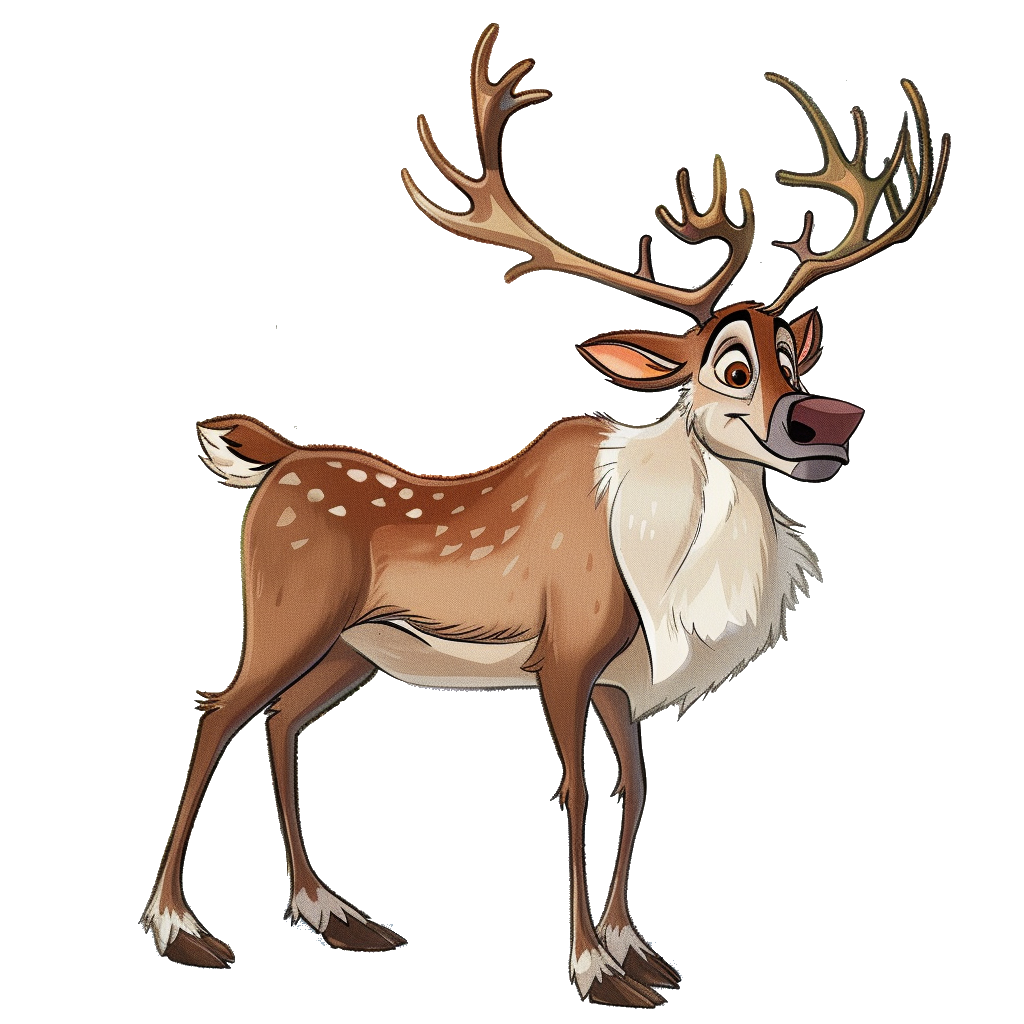
\includegraphics[width=0.3\linewidth]{05reindeersA.png}		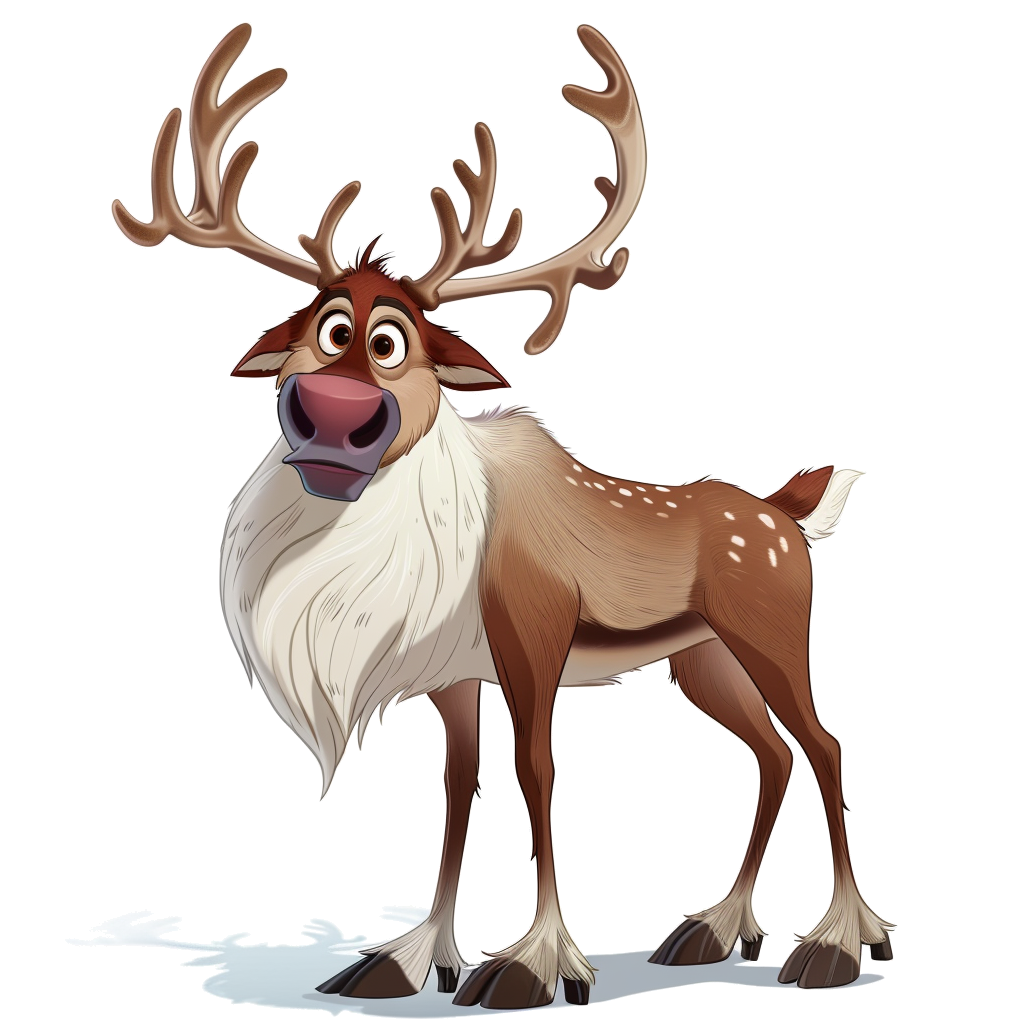
\includegraphics[width=0.3\linewidth]{05reindeersB.png}		
\includegraphics[width=0.3\linewidth]{05reindeersC.png}
	\end{center}
	
	% A: 1 1 36 => s=38
	% B: 1 2 18 => s=21
	% C: 1 3 12 => s=16
	% D: 1 4 9 => s=14
	% E: 1 6 6 => s=13
	% F: 2 2 9 => s=13
	% G: 2 3 6 => s=11
	% H: 3 3 4 => s=10
	
	% not enough info => E or F
	% eldest exists => F and eldest is 9 years old
	
	
	
\end{document}